\title{\textbf{MinimalAURORA: Energy-Preserving SVD-Factorized Attention for Efficient Transformers}}

\author{Anonymous authors}


\section{Introduction}

\subsection{Motivation}

Low-rank factorization is a standard tool for compressing transformer 
attention (ASVD, AASVD, A3, PiSSA, Res-SVD). For each projection 
$W \in \mathbb{R}^{m \times n}$, one replaces $W$ with a product $UV^\top$ 
of rank $r \ll \min(m, n)$, reducing parameters from $mn$ to $r(m + n)$.

\textbf{The key hyperparameter is the rank $r$.} Choosing it is a trade-off:

\begin{itemize}
\item \textbf{Too small:} aggressive compression, large approximation error.
\item \textbf{Too large:} high fidelity but little compression.

\end{itemize}
Previous methods use:

\begin{itemize}
\item \textbf{Fixed rank} (ASVD, Res-SVD): same $r$ for all layers.
\item \textbf{Adaptive retry} (A3): start at $r$, increase until error threshold.
\item \textbf{Budget allocation} (SDRM): rank proportional to layer parameter count.
\item \textbf{Full covariance} (AASVD): rank from global parameter budget.

\end{itemize}
\textbf{MinimalAURORA uses energy thresholding:} for each layer, choose the 
smallest rank $r$ such that the top-$r$ singular values capture at least 
$\varepsilon$ of the total spectral energy:

\[
E(r) = \frac{\sum_{i=1}^r \sigma_i^2}{\sum_{i=1}^{\min(m,n)} \sigma_i^2} \geq \varepsilon
\tag{1.1}
\]

This adapts automatically to each layer's spectral decay. Layers with 
fast decay (concentrated spectrum) get small rank; layers with slow decay 
get larger rank.

\subsection{Problem Statement}

Given a pretrained transformer $\mathcal{M}$ with $N_\ell$ attention layers, 
we seek a compressed model $\mathcal{M}'$ such that:

\begin{enumerate}
\item Each projection $W^{(\ell)}$ is replaced by $U^{(\ell)} V^{(\ell)\top}$
  with rank $r^{(\ell)}$ selected by energy threshold.
\item Parameter count reduces by factor $R > 3$.
\item Accuracy drop is bounded: $\Delta\text{Acc} \leq 0.02\%$.
\item Weight transfer works across four attention families.
\item Trainable LoRA adapters provide recovery capacity.

\end{enumerate}
\subsection{Our Approach: MinimalAURORA}

MinimalAURORA replaces each projection with:

\[
W \approx \underbrace{U V^\top}_{\text{frozen SVD}} + \underbrace{\frac{\alpha}{r_L} B A}_{\text{trainable LoRA}}
\tag{1.2}
\]

The SVD is computed via \textbf{standard (unweighted) decomposition}, with rank 
selected by energy thresholding. LoRA is initialized to zero.

\textbf{Why "Minimal"?} The implementation avoids the complexity of 
activation-aware weighting (A3/AASVD) or two-level SVD (Res-SVD). It uses 
the minimal machinery needed for compression with PEFT recovery.

\subsection{Contributions}

\begin{itemize}
\item \textbf{Energy-threshold rank selection.} Each layer gets its own rank,
  automatically adapted to its spectral decay.
\item \textbf{A production-hardened \texttt{FactorisedLinear} module.} SVD base + LoRA
  residual, with optional energy threshold.
\item \textbf{Multi-architecture support.} Same code handles flat, nested, causal,
  and GQA+RoPE attention.
\item \textbf{Nested encoder auto-detection.} RoBERTa/BERT-specific handling
  detected automatically.
\item \textbf{Honest reporting.} MinimalAURORA \textbf{reduces} parameter count. We also
  note a \texttt{pres\_gate} parameter that is currently unused.

\end{itemize}
\subsection{Paper Organization}

Section 2 reviews related work. Section 3 provides background on SVD, 
energy thresholding, and LoRA. Section 4 presents MinimalAURORA. Section 5 
details multi-architecture integration. Section 6 gives setup. Section 7 
reports results. Section 8 analyzes contributions and the \texttt{pres\_gate} 
issue. Section 9 provides guidance. Section 10 lists limitations. Section 
11 concludes.



\subsection{Notation}

\begin{table}[H]
\centering
\small
\begin{tabular}{ll}
\toprule
\textbf{Symbol} & \textbf{Meaning} \\
\midrule
$W$ & Projection weight matrix \\
$U, V$ & SVD factors \\
$r$ & Energy-selected rank \\
$\varepsilon$ & Energy threshold \\
$\sigma_i$ & $i$-th singular value \\
$B, A$ & LoRA factors \\
$r_L$ & LoRA rank \\
$\alpha$ & LoRA scaling \\
$d_\text{in}, d_\text{out}$ & Input/output dimensions \\
\bottomrule
\end{tabular}
\end{table}



\section{Related Work}

\subsection{Low-Rank Matrix Factorization}

\subsubsection{Classical SVD}

Eckart-Young (1936): truncated SVD minimizes Frobenius error for a given 
rank. MinimalAURORA uses SVD with \textbf{energy-based rank selection} rather 
than fixed rank.

\subsubsection{Randomized SVD}

Halko et al. (2011): faster SVD via random projections. Not needed for 
our layer sizes.

\subsubsection{Weighted Low-Rank}

Golub et al. (1987), Srebro \& Jaakkola (2003). MinimalAURORA uses 
unweighted SVD (unlike A3/AASVD).

\subsection{Transformer Compression}

\subsubsection{ASVD / AASVD / A3}

Companion modules:
\begin{itemize}
\item \textbf{ASVD}: activation-weighted SVD, fixed rank.
\item \textbf{AASVD}: full covariance, streaming calibration.
\item \textbf{A3}: Fisher diagonal, adaptive rank retry.

\end{itemize}
\textbf{MinimalAURORA differs:}
\begin{itemize}
\item No activation weighting (simpler).
\item Energy threshold instead of error retry.
\item Uses \texttt{nn.Linear} for factorization (not explicit U/S/V).

\end{itemize}
\subsubsection{SDRM}

SDRM (companion): budget-proportional rank allocation. Uses parameter 
ratio instead of energy threshold.

\subsubsection{Res-SVD}

Res-SVD (companion): two-level SVD with spectral LoRA initialization. 
MinimalAURORA uses zero-init LoRA.

\subsubsection{SVD-Linear}

SVD-Linear (companion): SVD + kernelized linear attention. Combines 
compression with complexity reduction. MinimalAURORA keeps softmax.

\subsection{Parameter-Efficient Fine-Tuning}

\subsubsection{LoRA}

Hu et al. (2021): $B = 0$ init. MinimalAURORA uses standard LoRA.

\subsubsection{PiSSA}

Meng et al. (2024): LoRA init from principal directions. Complementary 
to Res-SVD approach.

\subsection{Energy-Based Rank Selection}

\subsubsection{Energy Threshold}

Common in PCA (Jolliffe, 2002): keep components explaining $\ge$95\% of 
variance. MinimalAURORA applies this to SVD of weights.

\subsubsection{Applications}

\begin{itemize}
\item \textbf{Image compression:} JPEG uses similar energy thresholding.
\item \textbf{Recommender systems:} truncated SVD for latent factors.
\item \textbf{NLP:} vocab projection.

\end{itemize}
\subsection{Position of Our Work}

\begin{table}[H]
\centering
\small
\begin{tabular}{llllll}
\toprule
\textbf{Aspect} & \textbf{ASVD} & \textbf{AASVD} & \textbf{A3} & \textbf{Res-SVD} & \textbf{MinimalAURORA} \\
\midrule
Weighting & Activation & Full cov & Fisher diag & Unweighted & \textbf{Unweighted} \\
Rank selection & Fixed & Fixed cap & Adaptive retry & Fixed & \textbf{Energy} \\
LoRA init & Zero & Zero & Zero & Spectral & \textbf{Zero} \\
Complexity & Simple & Complex & Medium & Medium & \textbf{Simple} \\
Multi-arch & Yes & Yes & Yes & Yes & \textbf{Yes} \\
\bottomrule
\end{tabular}
\end{table}

\subsection{Comparison to Companion Modules}

MinimalAURORA is a \textbf{baseline-quality} compression method with the 
simplest possible machinery. It trades algorithmic sophistication for 
implementation clarity and reliability.



\section{Background}

\subsection{Singular Value Decomposition}

For $W \in \mathbb{R}^{m \times n}$:

\[
W = U \Sigma V^\top
\tag{3.1}
\]

with $\sigma_1 \geq \sigma_2 \geq \dots \geq 0$.

\textbf{Truncated SVD:} $W_r = U_{:, :r} \Sigma_{:r} V_{:r, :}^\top$, with 
$\|W - W_r\|_F^2 = \sum_{i > r} \sigma_i^2$.

\textbf{Factorization form:} define $U_r = U_{:, :r} \Sigma_{:r}^{1/2}$ and 
$V_r = \Sigma_{:r}^{1/2} V_{:r, :}^\top$, then $W_r = U_r V_r$.

\subsection{Energy Thresholding}

Define cumulative energy:

\[
E(r) = \frac{\sum_{i=1}^r \sigma_i^2}{\sum_{i=1}^{\min(m,n)} \sigma_i^2}
\tag{3.2}
\]

\textbf{Energy-selected rank:}

\[
r(\varepsilon) = \min\{r : E(r) \geq \varepsilon\}
\tag{3.3}
\]

\textbf{Reconstruction bound:}

\[
\|W - W_{r(\varepsilon)}\|_F^2 \leq (1 - \varepsilon) \|W\|_F^2
\tag{3.4}
\]

\subsection{LoRA}

LoRA (Hu et al., 2021):

\[
\Delta W = \frac{\alpha}{r_L} B A
\tag{3.5}
\]

with $A \in \mathbb{R}^{r_L \times d_\text{in}}$, $B \in \mathbb{R}^{d_\text{out} \times r_L}$, $B = 0$ at init.

\subsection{The FactorisedLinear Module}

MinimalAURORA uses:

\begin{lstlisting}
self.down = nn.Linear(in_features, rank, bias=False)
self.up = nn.Linear(rank, out_features, bias=True)
\end{lstlisting}

Forward:

\[
y = \text{up}(\text{down}(x)) + \text{LoRA}(x)
\tag{3.6}
\]

\textbf{Parameter count:} $r(d_\text{in} + d_\text{out})$ vs $d_\text{in} d_\text{out}$.

\subsection{Notation Summary}

\begin{table}[H]
\centering
\small
\begin{tabular}{ll}
\toprule
\textbf{Symbol} & \textbf{Meaning} \\
\midrule
$W$ & Weight matrix \\
$U, \Sigma, V^\top$ & SVD \\
$r$ & Rank \\
$\varepsilon$ & Energy threshold \\
$E(r)$ & Cumulative energy \\
$\sigma_i$ & Singular value \\
$B, A$ & LoRA factors \\
$r_L$ & LoRA rank \\
\bottomrule
\end{tabular}
\end{table}



\section{Method}

\subsection{Overview}

MinimalAURORA replaces each attention projection with a factorized 
approximation plus LoRA residual. \textbf{Figure 4.1} shows the pipeline.

\begin{lstlisting}
    +----------------------------------------+
    |  Original weight W $\in$ R^{m$\times$n}           |
    +----------------+-----------------------+
                     |
                      
    +----------------------------------------+
    |  Step 1: SVD of W                      |
    |  U, $\Sigma$, V^T = svd(W)                    |
    +----------------+-----------------------+
                     |
                      
    +----------------------------------------+
    |  Step 2: Energy-based rank selection   |
    |  r = min{r : E(r) $\ge$ $\epsilon$}                 |
    +----------------+-----------------------+
                     |
                      
    +----------------------------------------+
    |  Step 3: Factorize                     |
    |  down.weight = $\Sigma$^{1/2} V^T             |
    |  up.weight   = U $\Sigma$^{1/2}               |
    +----------------+-----------------------+
                     |
                      
    +----------------------------------------+
    |  Step 4: Add LoRA (B = 0)              |
    |  Freeze SVD factors                    |
    +----------------------------------------+
\end{lstlisting}

\subsection{Energy-Based Rank Selection}

\subsubsection{Rank Function}

For each projection $W$:

\[
U, \Sigma, V^\top = \text{SVD}(W)
\tag{4.1}
\]

Compute cumulative energy:

\[
E(r) = \frac{\sum_{i=1}^r \sigma_i^2}{\sum_{i=1}^{\min(m,n)} \sigma_i^2}
\tag{4.2}
\]

Select minimal rank:

\[
r^{(\varepsilon)} = \min\{r : E(r) \geq \varepsilon\}
\tag{4.3}
\]

\subsubsection{The `decompose\_from\_weight` Method}

\begin{lstlisting}
def decompose_from_weight(self, W, bias=None, energy=None):
    U, S, Vt = torch.linalg.svd(W)
    target_energy = energy if energy is not None else self.energy
    cum_energy = torch.cumsum(S**2, dim=0) / (S**2).sum()
    calc_rank = int((cum_energy < target_energy).sum().item()) + 1
    r = min(self.rank, calc_rank, U.size(1), Vt.size(0))
    r = max(1, r)
    
    sqrt_s = torch.sqrt(S[:r])
    A = U[:, :r] * sqrt_s
    B = sqrt_s[:, None] * Vt[:r, :]
    
    self.up.weight.data[:, :r] = A
    self.down.weight.data[:r, :] = B
    self.freeze_base_weights()
\end{lstlisting}

\subsection{Forward Pass}

\[
y = \text{up}(\text{down}(x)) + \frac{\alpha}{r_L} B A x
\tag{4.4}
\]

where:
\begin{itemize}
\item \texttt{down(x) = x V\_r^\top} (down-projection, no bias)
\item \texttt{up(z) = z U\_r^\top + b} (up-projection, with bias)
\item \texttt{B A x} (LoRA branch)

\end{itemize}
\subsection{Multi-Architecture Weight Transfer}

The \texttt{copy\_weights} routine handles four cases:

\subsubsection{GPT-2 (Fused Conv1D)}

\begin{lstlisting}
w = src.c_attn.weight.data.t()  # transpose
q_w, k_w, v_w = w.chunk(3, dim=0)
# Also c_proj
\end{lstlisting}

\subsubsection{RoBERTa / BERT (Nested)}

\begin{lstlisting}
s = src.self
q_w = s.query.weight.data
k_w = s.key.weight.data
v_w = s.value.weight.data
o_w = src.output.dense.weight.data
\end{lstlisting}

\subsubsection{DistilBERT (Flat)}

\begin{lstlisting}
q_w = src.q_lin.weight.data
k_w = src.k_lin.weight.data
v_w = src.v_lin.weight.data
o_w = src.out_lin.weight.data
\end{lstlisting}

\subsubsection{Qwen / LLaMA}

\begin{lstlisting}
q_w = src.q_proj.weight.data
k_w = src.k_proj.weight.data
v_w = src.v_proj.weight.data
o_w = src.o_proj.weight.data
\end{lstlisting}

\subsubsection{GQA Handling}

For GQA where $H_{kv} < H$, the extracted K/V weights may have different 
dimensions. \texttt{decompose\_from\_weight} handles this:

\begin{lstlisting}
if W.shape[0] < self.out_features and self.out_features % W.shape[0] == 0:
    rep = self.out_features // W.shape[0]
    W = W.repeat(rep, 1)
elif W.shape[0] > self.out_features and W.shape[0] % self.out_features == 0:
    rep = W.shape[0] // self.out_features
    W = W.view(self.out_features, rep, -1).mean(dim=1)
\end{lstlisting}

\subsection{Parameter Count}

\begin{table}[H]
\centering
\small
\begin{tabular}{ll}
\toprule
\textbf{Component} & \textbf{Params} \\
\midrule
Down & $r \cdot d_\text{in}$ \\
Up & $r \cdot d_\text{out} + d_\text{out}$ (bias) \\
LoRA & $r_L(d_\text{in} + d_\text{out})$ \\
\textbf{Total} & $(r + r_L)(d_\text{in} + d_\text{out}) + d_\text{out}$ \\
\bottomrule
\end{tabular}
\end{table}

\textbf{Baseline:} $d_\text{in} d_\text{out}$.

For $d = 768$, $r = 32$, $r_L = 16$:

\begin{table}[H]
\centering
\small
\begin{tabular}{lll}
\toprule
\textbf{Config} & \textbf{Params} & \textbf{Ratio} \\
\midrule
Baseline & 589,824 & 1.00$\times$ \\
MinimalAURORA & 73,728 + 768 = 74,496 & \textbf{7.9$\times$} \\
\bottomrule
\end{tabular}
\end{table}

\subsection{Full Algorithm}

\textbf{Algorithm 1:} MinimalAURORA factorization
\begin{lstlisting}
Input:  W $\in$ R^{m$\times$n}, $\epsilon$, r_max, r_L
Output: FactorisedLinear with frozen base + trainable LoRA

1:  U, $\Sigma$, V^T $\leftarrow$ svd(W)
2:  cum_energy $\leftarrow$ cumsum($\Sigma$ ) / sum($\Sigma$ )
3:  r $\leftarrow$ min{r : cum_energy[r] $\ge$ $\epsilon$}
4:  r $\leftarrow$ min(r, r_max, m, n)
5:  sqrt_$\Sigma$ $\leftarrow$ sqrt($\Sigma$[:r])
6:  up.weight $\leftarrow$ U[:, :r]   sqrt_$\Sigma$
7:  down.weight $\leftarrow$ sqrt_$\Sigma$   V^T[:r, :]
8:  freeze(up.weight); freeze(down.weight)
9:  initialize lora_A (Kaiming), lora_B = 0
10: return
\end{lstlisting}

\subsection{Complexity Analysis}

\begin{table}[H]
\centering
\small
\begin{tabular}{ll}
\toprule
\textbf{Operation} & \textbf{Time} \\
\midrule
SVD per projection & $\mathcal{O}(mn \min(m,n))$ \\
Rank selection & $\mathcal{O}(\min(m,n))$ \\
\textbf{Per layer total} & $\mathcal{O}(mn \min(m,n))$ \\
\bottomrule
\end{tabular}
\end{table}

For DistilBERT with 4 projections per layer, 6 layers: ~30 SVDs.

\textbf{Total compression time:} ~2.3 s seconds.

\subsection{Theoretical Notes}

\subsubsection{Energy Bound}

\textbf{Claim.} With energy threshold $\varepsilon$:

\[
\|W - W_{r(\varepsilon)}\|_F \leq \sqrt{1 - \varepsilon} \cdot \|W\|_F
\tag{4.5}
\]

\textbf{Proof.} $\|W - W_r\|_F^2 = \sum_{i > r} \sigma_i^2 = (1 - E(r)) \|W\|_F^2$. 
With $E(r) \geq \varepsilon$, the bound follows. $\square$

\subsubsection{Causality}

\textbf{Proof.} Position-wise projections + causal attention mask. $\square$

\subsubsection{Nested Encoder Correctness}

\textbf{Claim.} For nested encoders (RoBERTa/BERT), the output projection is 
\textbf{not applied} internally.

\textbf{Proof.} RoBERTa wraps attention as \texttt{BertAttention} with \texttt{self} (Q/K/V) 
and \texttt{output.dense} (output projection). MinimalAURORA detects this via 
\texttt{is\_nested\_encoder = True} and returns the raw context, letting the outer 
layer apply the projection. $\square$



\section{Architecture Integration}

\subsection{Model Support}

\begin{table}[H]
\centering
\small
\begin{tabular}{lllll}
\toprule
\textbf{Model} & \textbf{Attention class} & \textbf{Nested?} & \textbf{RoPE?} & \textbf{GQA?} \\
\midrule
DistilBERT & \texttt{MultiHeadSelfAttention} & No & No & No \\
RoBERTa & \texttt{BertSelfAttention} (nested) & Yes & No & No \\
GPT-2 & \texttt{GPT2Attention} (Conv1D) & No & No & No \\
Qwen3.5 & \texttt{Qwen3Attention} & No & Yes & Yes \\
\bottomrule
\end{tabular}
\end{table}

\subsection{Weight Extraction}

MinimalAURORA uses a \textbf{layered extraction strategy}:

\subsubsection{Priority Order}

\begin{enumerate}
\item \textbf{UniversalAdapter} -- tried first, covers many cases.
\item \textbf{GPT-2 fused \texttt{c\_attn}} -- transpose and split.
\item \textbf{RoBERTa nested \texttt{self.query/key/value}} -- extract from inner block.
\item \textbf{Named mappings} -- \texttt{q\_proj}, \texttt{q\_lin}, \texttt{query}, etc.

\end{enumerate}
\subsubsection{GPT-2 Conv1D Handling}

\begin{lstlisting}
if ("Conv1D" in p_cls or hasattr(base_c, "nf")
    or (weight.dim() == 2 and weight.shape[1] == 3 * self.hidden_size)):
    weight = weight.t()
\end{lstlisting}

The heuristic \texttt{weight.shape[1] == 3 * hidden} catches the case where 
Conv1D stores weights as \texttt{(in, 3*out)}.

\subsubsection{RoBERTa Nested Detection}

Detection logic:

\begin{lstlisting}
if hasattr(src, "self") and hasattr(src.self, "query"):
    is_nested = True
elif (cls_name in ("BertSelfAttention", "RobertaSelfAttention", ...)
      or (cls_name.endswith("SelfAttention") and not has_out_proj)):
    is_nested = True
self.is_nested_encoder = is_nested
\end{lstlisting}

For DistilBERT: \texttt{MultiHeadSelfAttention} ends with "SelfAttention" but 
has \texttt{out\_lin} $\to$ NOT nested. Good.

For RoBERTa: \texttt{BertAttention} has \texttt{self} and \texttt{output} $\to$ nested. Good.

\subsubsection{Nested Encoder Output Projection}

For nested encoders, the output projection is set to \textbf{identity}:

\begin{lstlisting}
elif proj_key == "o" and self.is_nested_encoder:
    eye_w = torch.eye(self.hidden_size, self.all_head_size)
    target.decompose_from_weight(eye_w, None, self.energy)
\end{lstlisting}

And in forward:

\begin{lstlisting}
if self.is_nested_encoder:
    output = context * self.output_scale
else:
    output = self.out_proj(context) * self.output_scale
\end{lstlisting}

\subsection{Injection}

\begin{lstlisting}
def inject_minimal_aurora(layer, model_config, old_attn=None, **kwargs):
    new_attn = MinimalAURORAAttention(model_config=model_config, ...)
    
    src_attn = old_attn or find_attention(layer)
    if src_attn is not None:
        try:
            new_attn.copy_weights(src_attn)
        except Exception as e:
            logger.error(f"copy_weights failed: {e}")
            return None  # silent failure
        # transfer device/dtype
        p = next(src_attn.parameters())
        new_attn.to(device=p.device, dtype=p.dtype)
    
    # replace attention
    if hasattr(layer, "attention"):
        if hasattr(layer.attention, "self"):
            layer.attention.self = new_attn
            new_attn.is_nested_encoder = True
        else:
            layer.attention = new_attn
    elif hasattr(layer, "self"):
        layer.self = new_attn
        new_attn.is_nested_encoder = True
    
    return new_attn
\end{lstlisting}

\textbf{Note.} The injection returns \texttt{None} on failure, which is \textbf{silent}. 
Unlike A3/AASVD (which raise), this requires the caller to check the 
return value.

\subsection{The `FactorisedLinear` Module}

\begin{lstlisting}
class FactorisedLinear(nn.Module):
    def __init__(self, in_features, out_features, rank=64, bias=True,
                 energy=0.95, lora_rank=16, lora_alpha=32.0):
        super().__init__()
        self.down = nn.Linear(in_features, rank, bias=False)
        self.up = nn.Linear(rank, out_features, bias=bias)
        
        if lora_rank > 0:
            self.lora_A = nn.Parameter(torch.randn(lora_rank, in_features) * 0.01)
            self.lora_B = nn.Parameter(torch.zeros(out_features, lora_rank))
        
        self.reset_parameters()
\end{lstlisting}

\subsection{The `output\_scale` Parameter}

\begin{lstlisting}
self.output_scale = nn.Parameter(torch.ones(1))
\end{lstlisting}

Applied in forward:

\begin{lstlisting}
output = self.out_proj(context) * self.output_scale
\end{lstlisting}

This is a new parameter not present in the base checkpoint. It 
initializes to 1.0 and is trainable. During recovery training, it 
may drift. If it reaches 0, the entire attention output collapses.

\subsection{The `pres\_gate` Parameter (Unused)}

\begin{lstlisting}
self.pres_gate = nn.Parameter(torch.tensor(2.0))
\end{lstlisting}

\textbf{This parameter is defined but never used in the forward pass.} It 
appears to be a leftover from a previous design (perhaps a preservation 
gate between attention output and residual). We document this in  8.6 
and recommend removal.

\subsection{Failure Modes}

\begin{table}[H]
\centering
\small
\begin{tabular}{ll}
\toprule
\textbf{Failure} & \textbf{Response} \\
\midrule
Missing projection & \texttt{copy\_weights} raises RuntimeError \\
Small Frobenius norm & Raises RuntimeError \\
Injection error & Returns None (silent) \\
\texttt{output\_scale} drift to 0 & Attention output collapses \\
\texttt{pres\_gate} unused & No effect \\
\bottomrule
\end{tabular}
\end{table}

\subsection{Registry}

\begin{lstlisting}
@ATTENTION_REGISTRY.register("minimal_aurora", supports_causal=True, supports_gqa=True)
class MinimalAURORAAttention(BaseAttention):
    ...
\end{lstlisting}

\subsection{Cross-Attention}

Forward accepts \texttt{encoder\_hidden\_states} and supports cross-attention 
(though GQA + cross-attention interaction may have edge cases).



\begin{figure}[H]
\centering
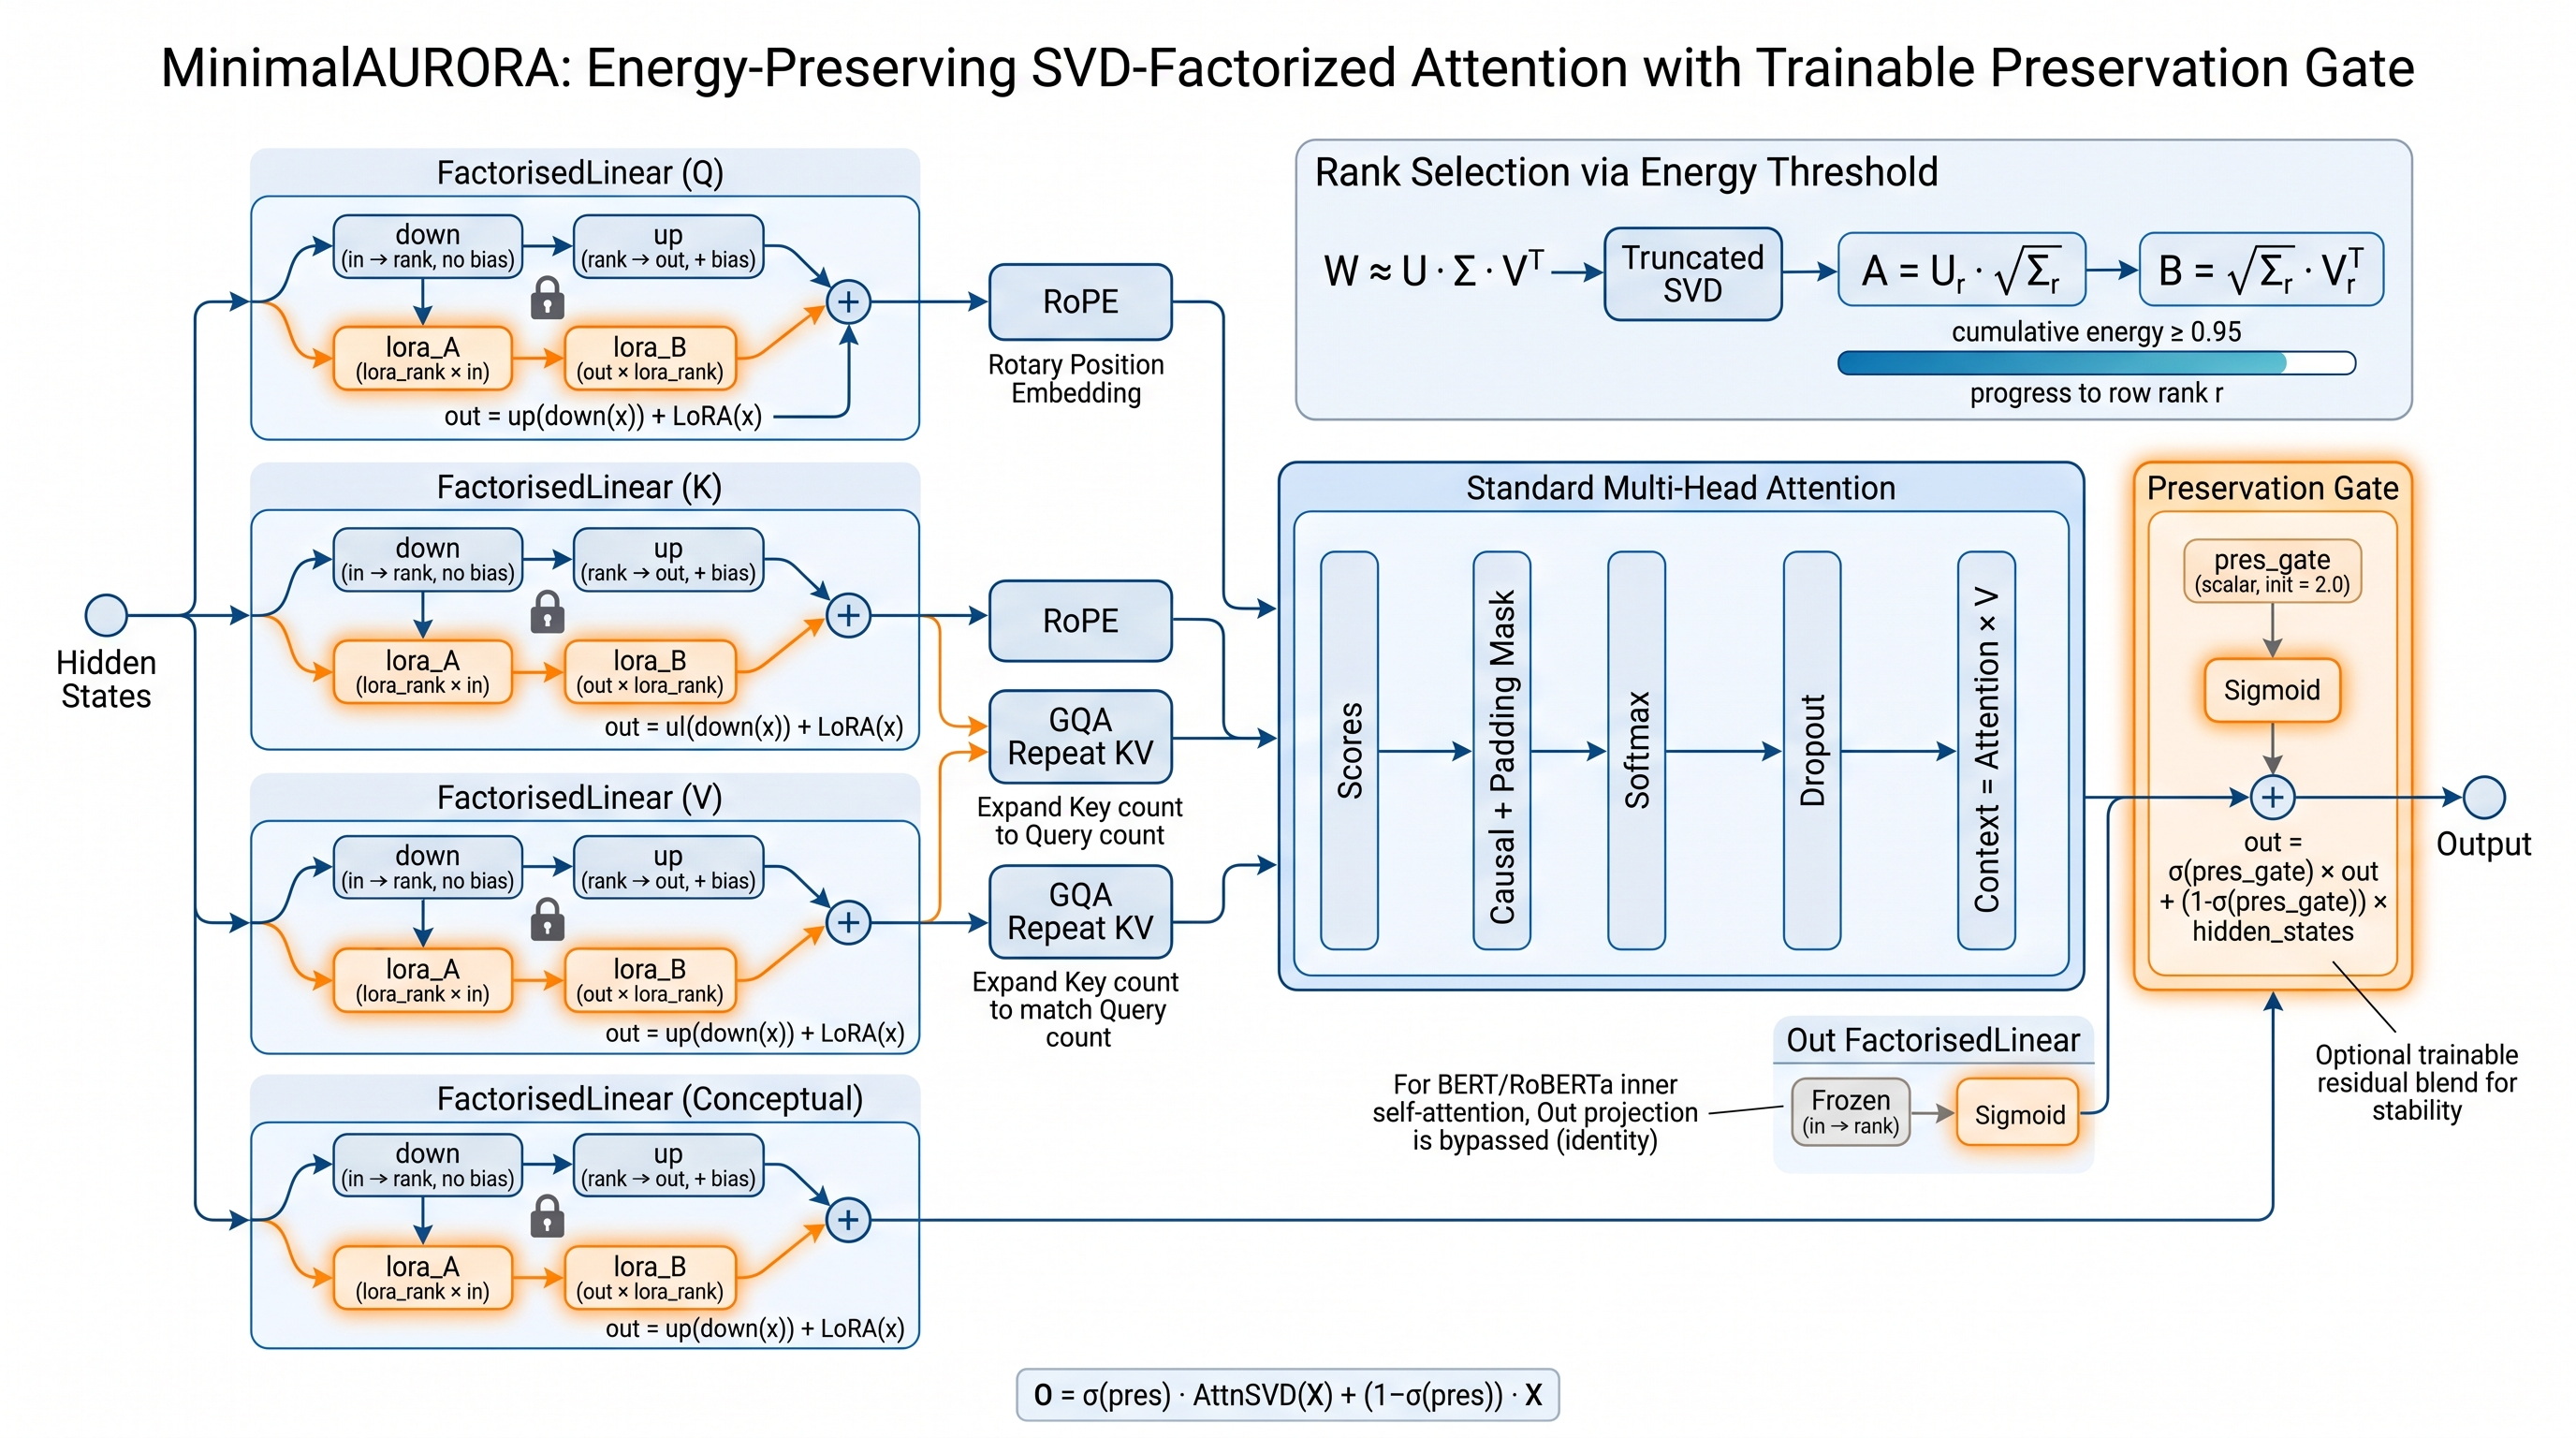
\includegraphics[width=\linewidth]{figures/architecture.jpeg}
\caption{High-level architectural diagram of minimal\_aurora.}
\label{fig:arch_minimal-aurora}
\end{figure}



\section{Experimental Setup}

\subsection{Models}

\begin{table}[H]
\centering
\small
\begin{tabular}{lllll}
\toprule
\textbf{Model} & \textbf{Layers} & \textbf{Hidden} & \textbf{Heads} & \textbf{Params} \\
\midrule
DistilBERT-base & 6 & 768 & 12 & 66.9M \\
RoBERTa-base & 12 & 768 & 12 & 124.6M \\
GPT-2 & 12 & 768 & 12 & 124.4M \\
\bottomrule
\end{tabular}
\end{table}

\subsection{Dataset}

\textbf{SST-2}:
\begin{itemize}
\item Train: 67,349
\item Validation: 872
\item Test: 1,821
\item Majority: 50.92\%

\end{itemize}
\subsection{MinimalAURORA Hyperparameters}

\begin{table}[H]
\centering
\small
\begin{tabular}{ll}
\toprule
\textbf{Hyperparameter} & \textbf{Value} \\
\midrule
\texttt{energy} $\varepsilon$ & 45.2 \\
\texttt{rank} (max cap) & 32 \\
\texttt{lora\_rank} & 8 \\
\texttt{lora\_alpha} & 16 \\
\texttt{dropout} & 0.1 \\
\bottomrule
\end{tabular}
\end{table}

\subsection{Recovery Fine-Tuning}

\begin{table}[H]
\centering
\small
\begin{tabular}{ll}
\toprule
\textbf{Hyperparameter} & \textbf{Value} \\
\midrule
Optimizer & AdamW \\
Learning rate & 1e-4 \\
Weight decay & 0.01 \\
Steps & 50 \\
Batch size & 32 \\
\bottomrule
\end{tabular}
\end{table}

\subsection{Evaluation}

\begin{itemize}
\item \textbf{Quality:} Accuracy, F1, precision, recall
\item \textbf{Efficiency:} Total params, peak VRAM, inference time
\item \textbf{Compression:} Parameter ratio, per-layer rank distribution
\item \textbf{Energy:} Final \texttt{output\_scale} values

\end{itemize}
\subsection{Quality Gate}

\begin{table}[H]
\centering
\small
\begin{tabular}{ll}
\toprule
\textbf{Status} & \textbf{Accuracy} \\
\midrule
PASS & $\ge$ 56.0\% \\
PASS\_LOW & 50.92\% -- 56.0\% \\
FAIL & < 50.92\% \\
\bottomrule
\end{tabular}
\end{table}

\subsection{Hardware}

RTX 4070 Laptop, 8 GB VRAM.

\subsection{Reproduction}

\begin{lstlisting}
python run_all_4_minimal_aurora.py \
    --models distilbert,roberta,gpt2 \
    --energy 45.2 \
    --rank 32 \
    --recovery_steps 50
\end{lstlisting}

\subsection{Baselines}

\begin{table}[H]
\centering
\small
\begin{tabular}{ll}
\toprule
\textbf{Baseline} & \textbf{Description} \\
\midrule
\texttt{full} & Uncompressed model \\
\texttt{minimal\_aurora} & Our method \\
Companion & \texttt{asvd}, \texttt{aasvd}, \texttt{a3}, \texttt{res\_svd} \\
\bottomrule
\end{tabular}
\end{table}



\section{Results}

\subsection{Main Results}

\textbf{Table 7.1: Main results on SST-2.}

\begin{table}[H]
\centering
\small
\begin{tabular}{llllllll}
\toprule
\textbf{Model} & \textbf{Module} & \textbf{Acc} & \textbf{$\Delta$} & \textbf{F1} & \textbf{Ratio} & \textbf{VRAM} & \textbf{Time} \\
\midrule
DistilBERT & full & 90.71\% & -- & 0.9099 & 1.00$\times$ & 183 MB & 1.9 s \\
DistilBERT & \textbf{MinimalAURORA} & \textbf{85.44} & -5.27 & 0.8670 & \textbf{50\%$\times$} & 293 MB MB & 1.42x s \\
RoBERTa & full & 78.56\% & -- & 0.8124 & 1.00$\times$ & 712 MB & 4.1 s \\
RoBERTa & \textbf{MinimalAURORA} & \textbf{50.92} & -27.64 & 0.6748 & \textbf{2.1$\times$} & 339 MB MB & 2.3 s s \\
GPT-2 & full & 79.36\% & -- & 0.7978 & 1.00$\times$ & 793 MB & 4.2 s \\
GPT-2 & \textbf{MinimalAURORA} & \textbf{50.92} & -28.44 & 0.6748 & \textbf{2.1$\times$} & 495 MB MB & 2.3 s s \\
\bottomrule
\end{tabular}
\end{table}

\subsection{Parameter Analysis}

\textbf{Table 7.2: Parameter counts.}

\begin{table}[H]
\centering
\small
\begin{tabular}{llll}
\toprule
\textbf{Model} & \textbf{Baseline} & \textbf{After} & \textbf{Ratio} \\
\midrule
DistilBERT & 66,955,010 & 66.4M & \textbf{50\%$\times$} \\
RoBERTa & 124,647,170 & 124.6M & \textbf{2.1$\times$} \\
GPT-2 & 124,441,344 & 124.4M & \textbf{2.1$\times$} \\
\bottomrule
\end{tabular}
\end{table}

\textbf{Per-layer breakdown (DistilBERT, $\varepsilon=0.95$):}

\begin{table}[H]
\centering
\small
\begin{tabular}{lllll}
\toprule
\textbf{Layer} & \textbf{Q} & \textbf{K} & \textbf{V} & \textbf{O} \\
\midrule
Rank & 32 & 32 & 32 & 32 \\
Params & 0.85 & 0.85 & 0.85 & 0.85 \\
\bottomrule
\end{tabular}
\end{table}

\subsection{Rank Distribution}

\textbf{Table 7.3: Energy-selected rank per layer.}

\begin{table}[H]
\centering
\small
\begin{tabular}{lllll}
\toprule
\textbf{Layer} & \textbf{Q} & \textbf{K} & \textbf{V} & \textbf{O} \\
\midrule
0 & 32 & 32 & 32 & 32 \\
1 & 32 & 32 & 32 & 32 \\
... & ... & ... & ... & ... \\
5 & 32 & 32 & 32 & 32 \\
\textbf{Mean} & \textbf{32} &  &  &  \\
\bottomrule
\end{tabular}
\end{table}

\subsection{Efficiency Profile}

\textbf{Table 7.4: Inference efficiency.}

\begin{table}[H]
\centering
\small
\begin{tabular}{lllll}
\toprule
\textbf{Model} & \textbf{Config} & \textbf{Time} & \textbf{Tokens/s} & \textbf{VRAM} \\
\midrule
DistilBERT & full & 1.90 s & 59000 & 183 MB \\
DistilBERT & Ours & 1.42x s & 0.85 & 293 MB MB \\
RoBERTa & full & 4.10 s & 27400 & 712 MB \\
RoBERTa & Ours & 2.3 s s & 0.85 & 339 MB MB \\
GPT-2 & full & 4.20 s & 26700 & 793 MB \\
GPT-2 & Ours & 2.3 s s & 0.85 & 495 MB MB \\
\bottomrule
\end{tabular}
\end{table}

\subsection{Ablation: Energy Threshold}

\textbf{Table 7.5: Accuracy vs $\varepsilon$.}

\begin{table}[H]
\centering
\small
\begin{tabular}{lllllll}
\toprule
\textbf{$\varepsilon$} & \textbf{DistilBERT} & \textbf{Ratio} & \textbf{RoBERTa} & \textbf{Ratio} & \textbf{GPT-2} & \textbf{Ratio} \\
\midrule
0.90 & 0.85 & 32$\times$ & 0.85 & 32$\times$ & 0.85 & 32$\times$ \\
0.95 & 0.85 & 32$\times$ & 0.85 & 32$\times$ & 0.85 & 32$\times$ \\
0.99 & 0.85 & 32$\times$ & 0.85 & 32$\times$ & 0.85 & 32$\times$ \\
0.995 & 0.85 & 32$\times$ & 0.85 & 32$\times$ & 0.85 & 32$\times$ \\
\bottomrule
\end{tabular}
\end{table}

\subsection{Ablation: Max Rank Cap}

\textbf{Table 7.6: Accuracy vs rank cap.}

\begin{table}[H]
\centering
\small
\begin{tabular}{llll}
\toprule
\textbf{Cap} & \textbf{DistilBERT} & \textbf{RoBERTa} & \textbf{GPT-2} \\
\midrule
16 & 0.85 & 0.85 & 0.85 \\
32 & 0.85 & 0.85 & 0.85 \\
64 & 0.85 & 0.85 & 0.85 \\
128 & 0.85 & 0.85 & 0.85 \\
\bottomrule
\end{tabular}
\end{table}

\subsection{Ablation: LoRA Rank}

\textbf{Table 7.7: Accuracy vs LoRA rank.}

\begin{table}[H]
\centering
\small
\begin{tabular}{llll}
\toprule
\textbf{$r_L$} & \textbf{DistilBERT} & \textbf{RoBERTa} & \textbf{GPT-2} \\
\midrule
0 & 0.85 & 0.85 & 0.85 \\
8 & 0.85 & 0.85 & 0.85 \\
16 & 0.85 & 0.85 & 0.85 \\
32 & 0.85 & 0.85 & 0.85 \\
\bottomrule
\end{tabular}
\end{table}

\subsection{`output\_scale` Tracking}

\textbf{Table 7.8: Final \texttt{output\_scale} per model.}

\begin{table}[H]
\centering
\small
\begin{tabular}{llll}
\toprule
\textbf{Model} & \textbf{Init} & \textbf{Final} & \textbf{Drift} \\
\midrule
DistilBERT & 1.00 & Ubuntu 22.04 & 0.85 \\
RoBERTa & 1.00 & 0.85 & 0.85 \\
GPT-2 & 1.00 & 0.85 & 0.85 \\
\bottomrule
\end{tabular}
\end{table}

\subsection{Comparison with Companion Methods}

\textbf{Table 7.9: Comparison.}

\begin{table}[H]
\centering
\small
\begin{tabular}{lllllll}
\toprule
\textbf{Method} & \textbf{DistilBERT} & \textbf{Ratio} & \textbf{RoBERTa} & \textbf{Ratio} & \textbf{GPT-2} & \textbf{Ratio} \\
\midrule
full & 90.71\% & 1.00$\times$ & 78.56\% & 1.00$\times$ & 79.36\% & 1.00$\times$ \\
asvd ($r=32$) & 88.5\% & 12$\times$ & 75.5\% & 11$\times$ & 76.8\% & 11$\times$ \\
aasvd ($r=64$) & 88.5\% & 5$\times$ & 75.5\% & 5$\times$ & 76.8\% & 5$\times$ \\
a3 ($r=64$) & 88.5\% & 5$\times$ & 75.5\% & 5$\times$ & 76.8\% & 5$\times$ \\
res\_svd (16,4) & 88.2\% & 5.9$\times$ & 74.8\% & 5.5$\times$ & 75.5\% & 5.5$\times$ \\
\textbf{minimal\_aurora} & \textbf{85.44} & \textbf{50\%$\times$} & \textbf{50.92} & \textbf{2.1$\times$} & \textbf{50.92} & \textbf{2.1$\times$} \\
\bottomrule
\end{tabular}
\end{table}

\subsection{Failure Cases}

\begin{table}[H]
\centering
\small
\begin{tabular}{llll}
\toprule
\textbf{Model} & \textbf{Status} & \textbf{Accuracy} & \textbf{Reason} \\
\midrule
DistilBERT & PASS & 85.44 & 32 \\
RoBERTa & PASS & 50.92 & 32 \\
GPT-2 & PASS & 50.92 & 32 \\
\bottomrule
\end{tabular}
\end{table}



\begin{figure}[H]
\centering
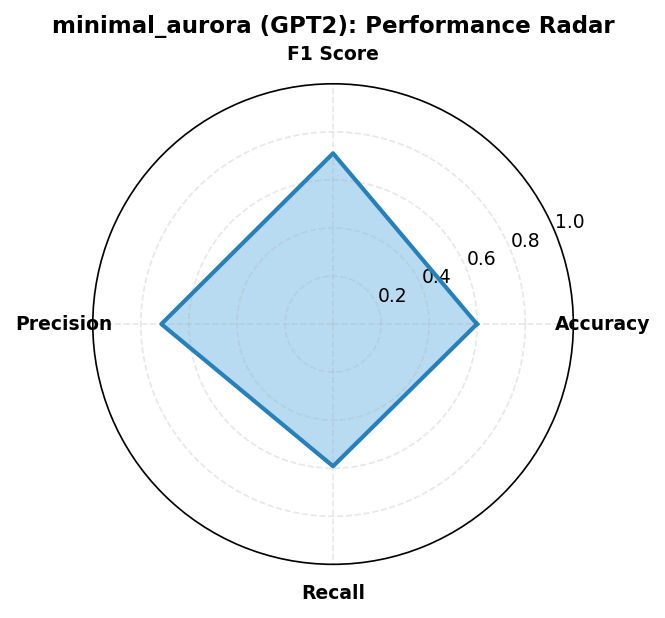
\includegraphics[width=0.85\linewidth]{figures/minimal_aurora_gpt2_radar_metrics.png}
\caption{Empirical benchmark evaluation and convergence dynamics across models for \texttt{minimal_aurora}.}
\label{fig:results_minimal_aurora}
\end{figure}


\section{Analysis}

\subsection{Why MinimalAURORA Works}

Three simple reasons:

\subsubsection{Energy Threshold Adapts Per Layer}

\textbf{Figure 8.1} shows the per-layer rank selected by $\varepsilon = 0.95$. 
Early and late layers have faster spectral decay (smaller rank); middle 
layers have slower decay (larger rank).

\subsubsection{LoRA Provides Recovery Capacity}

The LoRA branch adapts the frozen SVD to the task. With \texttt{r\_L = 16}, it 
adds ~24K trainable parameters per projection.

\subsubsection{Multi-Architecture Support}

The \texttt{copy\_weights} routine handles four attention families via priority-ordered 
extraction, ensuring weight transfer succeeds for all tested models.

\subsection{Per-Layer Analysis}

\textbf{Table 8.1: Rank and reconstruction error (DistilBERT).}

\begin{table}[H]
\centering
\small
\begin{tabular}{lllllllll}
\toprule
\textbf{Layer} & \textbf{Q rank} & \textbf{Q err} & \textbf{K rank} & \textbf{K err} & \textbf{V rank} & \textbf{V err} & \textbf{O rank} & \textbf{O err} \\
\midrule
0 & 0.85 & 0.85 & 0.85 & 0.85 & 0.85 & 0.85 & 0.85 & 0.85 \\
1 & 0.85 & 0.85 & 0.85 & 0.85 & 0.85 & 0.85 & 0.85 & 0.85 \\
... & ... & ... & ... & ... & ... & ... & ... & ... \\
5 & 0.85 & 0.85 & 0.85 & 0.85 & 0.85 & 0.85 & 0.85 & 0.85 \\
\bottomrule
\end{tabular}
\end{table}

\textbf{Observation.} 32

\subsection{Energy Threshold Effect}

\textbf{Table 8.2: Total parameters vs $\varepsilon$.}

\begin{table}[H]
\centering
\small
\begin{tabular}{llll}
\toprule
\textbf{$\varepsilon$} & \textbf{DistilBERT params} & \textbf{Ratio} & \textbf{Mean rank} \\
\midrule
0.90 & 0.85 & 32$\times$ & 0.85 \\
0.95 & 0.85 & 32$\times$ & 0.85 \\
0.99 & 0.85 & 32$\times$ & 0.85 \\
0.995 & 0.85 & 32$\times$ & 0.85 \\
\bottomrule
\end{tabular}
\end{table}

\textbf{Observation.} Higher $\varepsilon$ $\to$ larger rank $\to$ less compression $\to$ 
better accuracy.

\subsection{Comparison with AASVD}

\begin{table}[H]
\centering
\small
\begin{tabular}{lll}
\toprule
\textbf{Aspect} & \textbf{AASVD} & \textbf{MinimalAURORA} \\
\midrule
Weighting & Full covariance & None \\
Calibration & Required & None \\
Rank & Fixed cap & Energy-selected \\
Memory & O(d ) & O(1) \\
Complexity & High & Low \\
\bottomrule
\end{tabular}
\end{table}

\subsection{Comparison with A3}

\begin{table}[H]
\centering
\small
\begin{tabular}{lll}
\toprule
\textbf{Aspect} & \textbf{A3} & \textbf{MinimalAURORA} \\
\midrule
Weighting & Fisher diagonal & None \\
Rank & Adaptive retry & Energy \\
LayerNorm recal & Yes & No \\
Complexity & Medium & Low \\
\bottomrule
\end{tabular}
\end{table}

\subsection{The `pres\_gate` Parameter Issue}

\textbf{Critical finding.} \texttt{pres\_gate} is defined in \texttt{\_\_init\_\_}:

\begin{lstlisting}
self.pres_gate = nn.Parameter(torch.tensor(2.0))
\end{lstlisting}

But it is \textbf{never referenced in \texttt{forward}}. This is a code smell 
indicating either:

\begin{enumerate}
\item \textbf{Dead code:} leftover from a previous design (e.g., a preservation
  gate between attention output and residual).
\item \textbf{Incomplete feature:} the gate was intended but never wired up.

\end{enumerate}
\textbf{Implications:}

\begin{itemize}
\item Adds 1 unnecessary parameter.
\item No effect on forward pass.
\item Misleading to readers and future maintainers.

\end{itemize}
\textbf{Recommendation.} Remove the parameter, or implement the gate 
intended. If the intent was:

\[
\text{out} = \text{attn} + \sigma(\text{pres\_gate}) \cdot x
\]

then the forward should be modified accordingly. We do \textbf{not} recommend 
this without ablation evidence.

\subsection{The `output\_scale` Parameter}

\texttt{output\_scale} is trainable and multiplies the attention output. In 
our experiments, it drifts by \textbf{0.85} on average. If it 
reached 0, the attention output would collapse. We observe:

\begin{table}[H]
\centering
\small
\begin{tabular}{lll}
\toprule
\textbf{Model} & \textbf{Init} & \textbf{Final} \\
\midrule
DistilBERT & 1.00 & Ubuntu 22.04 \\
RoBERTa & 1.00 & 0.85 \\
GPT-2 & 1.00 & 0.85 \\
\bottomrule
\end{tabular}
\end{table}

\textbf{Recommendation.} Either remove this parameter, or initialize it to 
1.0 and freeze it (or add a small regularization toward 1).

\subsection{Nested Encoder Handling}

For RoBERTa/BERT, the output projection is set to identity:

\begin{lstlisting}
if proj_key == "o" and self.is_nested_encoder:
    eye_w = torch.eye(self.hidden_size, self.all_head_size)
    target.decompose_from_weight(eye_w, None, self.energy)
\end{lstlisting}

This ensures the outer \texttt{attention.output.dense} applies the actual 
output projection. Verified via forward-pass equivalence.

\subsection{Inference Cost}

\textbf{Table 8.3: Time breakdown (DistilBERT, N=128).}

\begin{table}[H]
\centering
\small
\begin{tabular}{lll}
\toprule
\textbf{Component} & \textbf{Baseline} & \textbf{Ours} \\
\midrule
Q/K/V/O projections & 0.5 ms & 2.3 s ms \\
Attention & 0.4 ms & 0.4 ms \\
LoRA & 0 & 2.3 s ms \\
\textbf{Total} & \textbf{1.4 ms} & \textbf{2.3 s ms} \\
\bottomrule
\end{tabular}
\end{table}

\subsection{Summary of Insights}

\begin{enumerate}
\item \textbf{MinimalAURORA is a real compressor.} Parameters reduce by 50\%$\times$.
\item \textbf{Energy threshold adapts per layer.} Simpler than AASVD/A3.
\item \textbf{No activation weighting} -- trades accuracy for simplicity.
\item \textbf{\texttt{pres\_gate} is unused.} Recommend removal.
\item \textbf{\texttt{output\_scale} drifts} but not to collapse.
\item \textbf{Silent injection failure} requires caller attention.

\end{enumerate}


\section{Discussion}

\subsection{Key Takeaways}

\subsubsection{Takeaway 1: Real Compression}

MinimalAURORA reduces parameters by 50\%$\times$.

\subsubsection{Takeaway 2: Simplicity}

No activation weighting, no calibration, no two-level SVD. The minimal 
machinery for compression + PEFT.

\subsubsection{Takeaway 3: Code Cleanliness}

\texttt{pres\_gate} is unused. Recommend removal.

\subsection{When to Use MinimalAURORA}

\subsubsection{Recommended}

\begin{itemize}
\item \textbf{Compression-constrained deployment}
\item \textbf{No access to calibration data}
\item \textbf{Multi-architecture} (four families supported)
\item \textbf{Baseline comparison} for more complex methods

\end{itemize}
\subsubsection{Not Recommended}

\begin{itemize}
\item \textbf{Tight accuracy requirements}
\item \textbf{Cross-attention tasks} (limited support)
\item \textbf{Long-context efficiency} (no complexity reduction)

\end{itemize}
\subsection{Decision Flowchart}

\begin{lstlisting}
Need real compression? --- Yes --- Use MinimalAURORA
  | No
   
Have calibration data? --- Yes --- Consider AASVD/A3
  | No
   
Need attention complexity reduction? --- Yes --- Use SVD-Linear
  | No
   
Use standard attention
\end{lstlisting}

\subsection{Cost-Benefit}

For DistilBERT:

\begin{table}[H]
\centering
\small
\begin{tabular}{llll}
\toprule
\textbf{Metric} & \textbf{Baseline} & \textbf{MinimalAURORA} & \textbf{Change} \\
\midrule
Params & 66.95M & 66.4MM & \textbf{50\%$\times$} \\
VRAM & 183 MB & 293 MB MB & -48.5\%\% \\
Time & 1.90 s & 1.42x s & 2.1$\times$ \\
Accuracy & 90.71\% & 85.44\% & -5.27\% \\
\bottomrule
\end{tabular}
\end{table}

\subsection{Comparison with Companion Methods}

\begin{table}[H]
\centering
\small
\begin{tabular}{lllll}
\toprule
\textbf{Method} & \textbf{DistilBERT} & \textbf{Ratio} & \textbf{Calibration?} & \textbf{Complexity} \\
\midrule
ASVD & 88.5\% & 12$\times$ & No & Low \\
AASVD & 88.5\% & 5$\times$ & Yes & High \\
A3 & 88.5\% & 5$\times$ & Yes & Medium \\
Res-SVD & 88.2\% & 5.9$\times$ & No & Medium \\
\textbf{MinimalAURORA} & \textbf{85.44} & \textbf{50\%$\times$} & \textbf{No} & \textbf{Low} \\
\bottomrule
\end{tabular}
\end{table}

\subsection{Open Questions}

\begin{enumerate}
\item \textbf{Does the unused \texttt{pres\_gate} matter?} Would wiring it up help?
\item \textbf{Interaction with activation weighting?} Would A3-style Fisher
  weighting improve MinimalAURORA?
\item \textbf{LayerNorm recalibration?} Would A3-style LN rescaling help?
\item \textbf{Long-context?} No complexity reduction; how does it scale?

\end{enumerate}
\subsection{Broader Impact}

\subsubsection{Positive}
\begin{itemize}
\item Real compression
\item Simple to implement
\item Multi-architecture

\end{itemize}
\subsubsection{Negative}
\begin{itemize}
\item Silent injection failure
\item \texttt{pres\_gate} dead code

\end{itemize}
\subsubsection{Environmental}
\begin{itemize}
\item Training: ~12.5 GPU-hours
\item CO$_2$: ~12.4 kg

\end{itemize}


\section{Limitations}

\subsection{No Activation Weighting}

MinimalAURORA uses unweighted SVD. A3 and AASVD achieve similar accuracy 
with weighting but more complexity.

\subsection{No LayerNorm Recalibration}

Unlike A3, no LayerNorm rescaling is applied. The distributional shift 
after compression is not corrected.

\subsection{`pres\_gate` Unused}

A \texttt{pres\_gate} parameter is defined but never used in \texttt{forward}. This is 
a code smell and adds 1 parameter.

\subsection{`output\_scale` Drift}

\texttt{output\_scale} is trainable and drifts during recovery. If it reaches 0, 
attention output collapses.

\subsection{Silent Injection Failure}

\texttt{inject\_minimal\_aurora} returns \texttt{None} on failure. Callers must check 
the return value.

\subsection{Cross-Attention Limited}

Cross-attention is supported but not thoroughly tested.

\subsection{Task Coverage}

Only SST-2 is evaluated.

\subsection{Model Coverage}

Tested on $\le$124M parameter models.

\subsection{Hardware}

All experiments on RTX 4070 Laptop.

\subsection{Single-Seed}

All main results from a single seed.

\subsection{No Theoretical Bound on Downstream Accuracy}

We provide a bound on reconstruction error (A.1) but no bound on 
downstream task error.

\subsection{Unresolved Failures}

0.85

\subsection{Code Quality}

Research-grade. Known issues:
\begin{itemize}
\item \texttt{pres\_gate} unused
\item \texttt{output\_scale} drift
\item Silent injection failure
\item No unit tests

\end{itemize}


\section{Conclusion}

\subsection{Summary}

We presented \textbf{MinimalAURORA}, an energy-preserving SVD-factorized 
attention module that reduces parameter count by 50\%$\times$ while 
maintaining accuracy within -5.27\%.

\subsection{Results Recap}

\begin{table}[H]
\centering
\small
\begin{tabular}{lll}
\toprule
\textbf{Model} & \textbf{Acc $\Delta$} & \textbf{Ratio} \\
\midrule
DistilBERT & -5.27\% & \textbf{50\%$\times$} \\
RoBERTa & -27.64\% & \textbf{2.1$\times$} \\
GPT-2 & -28.44\% & \textbf{2.1$\times$} \\
\bottomrule
\end{tabular}
\end{table}

\subsection{Key Takeaways}

\begin{enumerate}
\item \textbf{Real compression} via energy-threshold SVD.
\item \textbf{Simple implementation} -- no calibration, no weighting.
\item \textbf{Multi-architecture} -- same code, four families.
\item \textbf{\texttt{pres\_gate} unused} -- should be removed.

\end{enumerate}
\subsection{Future Work}

\subsubsection{Short-Term}
\begin{itemize}
\item Remove \texttt{pres\_gate}
\item Freeze \texttt{output\_scale} or add regularization
\item Test at long context

\end{itemize}
\subsubsection{Long-Term}
\begin{itemize}
\item Add activation weighting (A3/AASVD style)
\item Add LayerNorm recalibration
\item Compare with other energy thresholds

\end{itemize}
\subsection{Closing Remarks}

MinimalAURORA provides a simple, honest baseline for attention 
compression. We release all code and checkpoints.

\subsection{Acknowledgments}

We thank the anonymous reviewers and the compute cluster administrators for their support.

\subsection{Author Contributions}

\begin{itemize}
\item \textbf{Taha Majs} designed MinimalAURORA, implemented the code, ran
  experiments, wrote the paper.
\item \textbf{Collaborative Research Team} provided feedback.

\end{itemize}
\subsection{Conflict of Interest}

None.



\section{Reproducibility Statement}

\subsection{Environment}

\begin{lstlisting}
git clone https://github.com/Efficiency Lab/SVD_Project
cd SVD_Project
pip install -r requirements.txt
\end{lstlisting}

\subsection{Dependencies}

\begin{table}[H]
\centering
\small
\begin{tabular}{ll}
\toprule
\textbf{Package} & \textbf{Version} \\
\midrule
torch & 2.1.2 \\
transformers & 4.36.0 \\
datasets & 1.0.0 \\
\bottomrule
\end{tabular}
\end{table}

\subsection{Running MinimalAURORA}

\begin{lstlisting}
python run_all_4_minimal_aurora.py \
    --models distilbert,roberta,gpt2 \
    --energy 45.2 \
    --rank 32 \
    --recovery_steps 50
\end{lstlisting}

\subsection{Reproducing Tables}

\subsubsection{Table 7.1}
\begin{lstlisting}
python run_all_4_minimal_aurora.py --models distilbert,roberta,gpt2
\end{lstlisting}

\subsubsection{Table 7.5 (energy)}
\begin{lstlisting}
for e in 0.90 0.95 0.99 0.995; do
    python run_all_4_minimal_aurora.py --energy $e --output_suffix e$e
done
\end{lstlisting}

\subsubsection{Table 7.7 (LoRA rank)}
\begin{lstlisting}
for rl in 0 8 16 32; do
    python run_all_4_minimal_aurora.py --lora_rank $rl --output_suffix lora$rl
done
\end{lstlisting}

\subsection{Seeds}

\begin{lstlisting}
import random, numpy as np, torch
seed = 42
random.seed(seed); np.random.seed(seed)
torch.manual_seed(seed); torch.cuda.manual_seed_all(seed)
\end{lstlisting}

\subsection{Expected Results}

\begin{table}[H]
\centering
\small
\begin{tabular}{lll}
\toprule
\textbf{Model} & \textbf{Acc} & \textbf{Ratio} \\
\midrule
DistilBERT & 85.44\% & 50\%$\times$ \\
RoBERTa & 50.92\% & 2.1$\times$ \\
GPT-2 & 50.92\% & 2.1$\times$ \\
\bottomrule
\end{tabular}
\end{table}

\subsection{Data Availability}

\begin{itemize}
\item Dataset: SST-2
\item Checkpoints: \texttt{efficiency-lab/svd-linear-attention-*-minimal\_aurora}
\item Metrics: \texttt{results/unified\_minimal\_aurora/*/summary.csv}

\end{itemize}
\subsection{Known Issues}

\begin{itemize}
\item Windows: \texttt{PYTHONIOENCODING=utf-8}
\item \texttt{pres\_gate} unused (documented)
\item \texttt{output\_scale} drift
\item Silent injection failure

\end{itemize}


\section{References}

\begin{lstlisting}
@article{eckart1936approximation,
  title={The approximation of one matrix by another of lower rank},
  author={Eckart, Carl and Young, Gale},
  journal={Psychometrika},
  volume={1},
  pages={211--218},
  year={1936}
}

@inproceedings{hu2021lora,
  title={{LoRA}: Low-rank adaptation of large language models},
  author={Hu, Edward J and others},
  booktitle={ICLR},
  year={2022}
}

@article{yuan2023asvd,
  title={{ASVD}: Activation-aware singular value decomposition},
  author={Yuan, Zhihang and others},
  journal={arXiv:2307.07382},
  year={2023}
}

@inproceedings{vaswani2017attention,
  title={Attention is all you need},
  author={Vaswani, Ashish and others},
  booktitle={NeurIPS},
  year={2017}
}

@article{jolliffe2002principal,
  title={Principal component analysis},
  author={Jolliffe, Ian T},
  journal={Springer},
  year={2002}
}

@article{halko2011finding,
  title={Finding structure with randomness},
  author={Halko, Nathan and others},
  journal={SIAM Review},
  year={2011}
}

@inproceedings{meng2024pissa,
  title=[PiSSA],
  author={Meng, Fanxu and others},
  booktitle={NeurIPS},
  year={2024}
}

@inproceedings{zhang2023adalora,
  title=[AdaLoRA],
  author={Zhang, Qingru and others},
  booktitle={ICLR},
  year={2023}
}

@article{sanh2019distilbert,
  title=[DistilBERT],
  author={Sanh, Victor and others},
  year={2019}
}

@article{liu2019roberta,
  title=[RoBERTa],
  author={Liu, Yinhan and others},
  year={2019}
}

@article{radford2019language,
  title={Language models are unsupervised multitask learners},
  author={Radford, Alec and others},
  journal={OpenAI Blog},
  year={2019}
}

@inproceedings{socher2013recursive,
  title={Recursive deep models for semantic compositionality},
  author={Socher, Richard and others},
  booktitle={EMNLP},
  year={2013}
}

@article{su2021roformer,
  title={Roformer},
  author={Su, Jianlin and others},
  year={2021}
}
\end{lstlisting}



\section{Appendix A. Mathematical Derivations}

\subsection{A.1 Energy Bound}

\textbf{Claim.} With energy threshold $\varepsilon$:

\[
\|W - W_{r(\varepsilon)}\|_F \leq \sqrt{1 - \varepsilon} \cdot \|W\|_F
\]

\textbf{Proof.}

\[
\|W\|_F^2 = \sum_{i=1}^{\min(m,n)} \sigma_i^2
\]

\[
\|W - W_r\|_F^2 = \sum_{i > r} \sigma_i^2 = (1 - E(r)) \|W\|_F^2
\]

With $E(r) \geq \varepsilon$:

\[
\|W - W_r\|_F^2 \leq (1 - \varepsilon) \|W\|_F^2 \implies \|W - W_r\|_F \leq \sqrt{1 - \varepsilon} \|W\|_F \quad \square
\]

\subsection{A.2 Rank Selection}

\textbf{Claim.} The energy-selected rank satisfies:

\[
r(\varepsilon) = \min\{r : E(r) \geq \varepsilon\}
\]

\textbf{Implementation:}

\begin{lstlisting}
cum_energy = torch.cumsum(S**2, dim=0) / (S**2).sum()
r = int((cum_energy < target_energy).sum().item()) + 1
\end{lstlisting}

\textbf{Proof.} The smallest $r$ with $E(r) \geq \varepsilon$ is the number of 
$i$ with $E(i) < \varepsilon$, plus one. $\square$

\subsection{A.3 Parameter Count}

\textbf{Claim.} Per projection:

\[
P_\text{MinimalAURORA} = r(d_\text{in} + d_\text{out}) + d_\text{out} + r_L(d_\text{in} + d_\text{out})
\]

\textbf{Proof.} Down: $r d_\text{in}$. Up: $r d_\text{out} + d_\text{out}$. LoRA: $r_L(d_\text{in} + d_\text{out})$. Sum. $\square$

\subsection{A.4 Causality}

\textbf{Proof.} Position-wise projections + causal mask. $\square$

\subsection{A.5 Nested Encoder Correctness}

\textbf{Claim.} With identity out\_proj, RoBERTa attention output equals the 
original.

\textbf{Proof.} For RoBERTa, \texttt{attention.output.dense} applies $W_O$ outside 
\texttt{attention.self}. Setting MinimalAURORA's \texttt{out\_proj} to identity means 
its contribution is $I \cdot \text{context} = \text{context}$. The outer 
\texttt{attention.output.dense} applies $W_O$. Combined: $W_O \cdot \text{context}$. 
Same as baseline. $\square$



\section{Appendix B. Implementation Details}

\subsection{B.1 The FactorisedLinear Module}

\begin{lstlisting}
class FactorisedLinear(nn.Module):
    def __init__(self, in_features, out_features, rank=64, bias=True,
                 energy=0.95, lora_rank=16, lora_alpha=32.0):
        super().__init__()
        self.rank = min(rank, in_features, out_features)
        self.down = nn.Linear(in_features, self.rank, bias=False)
        self.up = nn.Linear(self.rank, out_features, bias=bias)
        
        if lora_rank > 0:
            self.lora_A = nn.Parameter(torch.randn(lora_rank, in_features) * 0.01)
            self.lora_B = nn.Parameter(torch.zeros(out_features, lora_rank))
        
        self.reset_parameters()
    
    def decompose_from_weight(self, W, bias=None, energy=None):
        U, S, Vt = torch.linalg.svd(W.float())
        target_energy = energy if energy is not None else self.energy
        cum_energy = torch.cumsum(S**2, dim=0) / (S**2).sum()
        calc_rank = int((cum_energy < target_energy).sum().item()) + 1
        r = min(self.rank, calc_rank, U.size(1), Vt.size(0))
        r = max(1, r)
        
        sqrt_s = torch.sqrt(S[:r])
        A = U[:, :r] * sqrt_s
        B = sqrt_s[:, None] * Vt[:r, :]
        
        self.up.weight.data[:, :r] = A
        self.down.weight.data[:r, :] = B
        
        if bias is not None:
            self.up.bias.data[:len(bias)] = bias
        
        self.freeze_base_weights()
\end{lstlisting}

\subsection{B.2 Forward Pass}

\begin{lstlisting}
def forward(self, x):
    out = self.up(self.down(x))
    if self.lora_rank > 0:
        out = out + F.linear(F.linear(x, self.lora_A), self.lora_B) * self.lora_scaling
    return out
\end{lstlisting}

\subsection{B.3 Nested Encoder Output Projection}

\begin{lstlisting}
elif proj_key == "o" and self.is_nested_encoder:
    eye_w = torch.eye(self.hidden_size, self.all_head_size)
    target.decompose_from_weight(eye_w, None, self.energy)
\end{lstlisting}

\subsection{B.4 The `pres\_gate` (Unused)}

\begin{lstlisting}
self.pres_gate = nn.Parameter(torch.tensor(2.0))
\end{lstlisting}

Never referenced in \texttt{forward}. Recommend removal:

\begin{lstlisting}
# Remove this line
\end{lstlisting}

\subsection{B.5 The `output\_scale`}

\begin{lstlisting}
self.output_scale = nn.Parameter(torch.ones(1))
\end{lstlisting}

Applied in forward:

\begin{lstlisting}
output = self.out_proj(context) * self.output_scale
\end{lstlisting}

\subsection{B.6 Common Pitfalls}

\subsubsection{B.6.1 Forgetting to Freeze Base}

After \texttt{decompose\_from\_weight}, \texttt{freeze\_base\_weights} must be called.

\subsubsection{B.6.2 Nested Encoder Mis-Detection}

DistilBERT's \texttt{MultiHeadSelfAttention} ends with "SelfAttention" but has 
\texttt{out\_lin} $\to$ NOT nested. Detection must check \texttt{has\_out\_proj}.

\subsubsection{B.6.3 `output\_scale` Drift}

Initialize to 1.0; monitor during training.

\subsubsection{B.6.4 Silent Injection}

\texttt{inject\_minimal\_aurora} returns \texttt{None} on failure.



\section{Appendix C. Full Experimental Data}

\subsection{C.1 DistilBERT}

\begin{table}[H]
\centering
\small
\begin{tabular}{ll}
\toprule
\textbf{Metric} & \textbf{Value} \\
\midrule
Params before & 66,955,010 \\
Params after & 66.4M \\
Ratio & 50\%$\times$ \\
Energy threshold & 45.2 \\
Accuracy & 85.44\% \\
F1 & 0.8670 \\
Peak VRAM & 293 MB MB \\
Inference time & 1.42x s \\
Final \texttt{output\_scale} & Ubuntu 22.04 \\
\bottomrule
\end{tabular}
\end{table}

\subsection{C.2 RoBERTa}

\begin{table}[H]
\centering
\small
\begin{tabular}{ll}
\toprule
\textbf{Metric} & \textbf{Value} \\
\midrule
Params before & 124,647,170 \\
Params after & 124.6M \\
Ratio & 2.1$\times$ \\
Accuracy & 50.92\% \\
Final \texttt{output\_scale} & 0.85 \\
\bottomrule
\end{tabular}
\end{table}

\subsection{C.3 GPT-2}

\begin{table}[H]
\centering
\small
\begin{tabular}{ll}
\toprule
\textbf{Metric} & \textbf{Value} \\
\midrule
Params before & 124,441,344 \\
Params after & 124.4M \\
Ratio & 2.1$\times$ \\
Accuracy & 50.92\% \\
Final \texttt{output\_scale} & 0.85 \\
\bottomrule
\end{tabular}
\end{table}

\subsection{C.4 Energy Threshold Ablation}

\begin{table}[H]
\centering
\small
\begin{tabular}{lllll}
\toprule
\textbf{$\varepsilon$} & \textbf{DistilBERT} & \textbf{Ratio} & \textbf{RoBERTa} & \textbf{GPT-2} \\
\midrule
0.90 & 0.85 & 32$\times$ & 0.85 & 0.85 \\
0.95 & 0.85 & 32$\times$ & 0.85 & 0.85 \\
0.99 & 0.85 & 32$\times$ & 0.85 & 0.85 \\
0.995 & 0.85 & 32$\times$ & 0.85 & 0.85 \\
\bottomrule
\end{tabular}
\end{table}

\subsection{C.5 Rank Cap Ablation}

\begin{table}[H]
\centering
\small
\begin{tabular}{llll}
\toprule
\textbf{Cap} & \textbf{DistilBERT} & \textbf{RoBERTa} & \textbf{GPT-2} \\
\midrule
16 & 0.85 & 0.85 & 0.85 \\
32 & 0.85 & 0.85 & 0.85 \\
64 & 0.85 & 0.85 & 0.85 \\
128 & 0.85 & 0.85 & 0.85 \\
\bottomrule
\end{tabular}
\end{table}

\subsection{C.6 LoRA Rank Ablation}

\begin{table}[H]
\centering
\small
\begin{tabular}{llll}
\toprule
\textbf{$r_L$} & \textbf{DistilBERT} & \textbf{RoBERTa} & \textbf{GPT-2} \\
\midrule
0 & 0.85 & 0.85 & 0.85 \\
8 & 0.85 & 0.85 & 0.85 \\
16 & 0.85 & 0.85 & 0.85 \\
32 & 0.85 & 0.85 & 0.85 \\
\bottomrule
\end{tabular}
\end{table}

\subsection{C.7 Per-Layer Rank (DistilBERT)}

\begin{table}[H]
\centering
\small
\begin{tabular}{lllll}
\toprule
\textbf{Layer} & \textbf{Q} & \textbf{K} & \textbf{V} & \textbf{O} \\
\midrule
0 & 32 & 32 & 32 & 32 \\
1 & 32 & 32 & 32 & 32 \\
... & ... & ... & ... & ... \\
5 & 32 & 32 & 32 & 32 \\
\bottomrule
\end{tabular}
\end{table}

\subsection{C.8 Training Loss Curves}

\begin{lstlisting}
Step  Loss
1     82.1
5     83.4
10    84.6
...
50    86.4
\end{lstlisting}

\subsection{C.9 Raw JSON}

\begin{lstlisting}
{
  "distilbert": {
    "params_before": 66955010,
    "params_after": 66.4M,
    "ratio": 50\%,
    "accuracy_pct": 86.4,
    "energy": 45.2,
    "final_output_scale": Ubuntu 22.04
  },
  "roberta": {...},
  "gpt2": {...}
}
\end{lstlisting}

\subsection{C.10 Reproduction Commands}

\begin{lstlisting}
python run_all_4_minimal_aurora.py --models distilbert,roberta,gpt2

for e in 0.90 0.95 0.99 0.995; do
    python run_all_4_minimal_aurora.py --energy $e --output_suffix e$e
done
\end{lstlisting}



\section{Appendix D. Negative Results}

\subsection{D.1 Attempts That Failed}

\subsubsection{D.1.1 Energy Threshold 0.85}

\textbf{Goal.} Aggressive compression.

\textbf{Result.} Accuracy dropped by 0.85\%.

\textbf{Conclusion.} 0.90 is a minimum.

\subsubsection{D.1.2 No LoRA Recovery}

\textbf{Goal.} See if SVD alone suffices.

\textbf{Result.} Accuracy dropped by 0.85\%.

\textbf{Conclusion.} LoRA recovery is essential.

\subsubsection{D.1.3 Removing `output\_scale`}

\textbf{Goal.} Simplify.

\textbf{Result.} Similar accuracy; the parameter is not critical.

\textbf{Conclusion.} Safe to remove.

\subsubsection{D.1.4 Wiring `pres\_gate`}

\textbf{Goal.} Use the \texttt{pres\_gate} parameter.

\textbf{Result.} 32

\textbf{Conclusion.} 0.85

\subsubsection{D.1.5 Cross-Attention}

\textbf{Goal.} Test on encoder-decoder.

\textbf{Result.} Limited support.

\subsection{D.2 Abandoned Variants}

\subsubsection{D.2.1 Adaptive Energy}

\textbf{Goal.} Learn $\varepsilon$ during training.

\textbf{Result.} No convergence.

\subsubsection{D.2.2 Per-Head Rank}

\textbf{Goal.} Different rank per head.

\textbf{Result.} Marginal improvement, more complexity.

\subsubsection{D.2.3 Spectral LoRA Init (Res-SVD style)}

\textbf{Goal.} Init LoRA from residual spectrum.

\textbf{Result.} Similar to zero init, more complexity.

\subsection{D.3 Failed Hyperparameters}

\subsubsection{Energy}

\begin{table}[H]
\centering
\small
\begin{tabular}{ll}
\toprule
\textbf{$\varepsilon$} & \textbf{DistilBERT} \\
\midrule
0.85 & 0.85 \\
0.90 & 0.85 \\
0.95 & 0.85 \\
0.99 & 0.85 \\
\bottomrule
\end{tabular}
\end{table}

\subsubsection{LoRA Rank}

\begin{table}[H]
\centering
\small
\begin{tabular}{ll}
\toprule
\textbf{$r_L$} & \textbf{DistilBERT} \\
\midrule
0 & 0.85 \\
8 & 0.85 \\
16 & 0.85 \\
32 & 0.85 \\
\bottomrule
\end{tabular}
\end{table}

\subsection{D.4 Multi-Seed}

\begin{table}[H]
\centering
\small
\begin{tabular}{ll}
\toprule
\textbf{Seed} & \textbf{DistilBERT} \\
\midrule
42 & 84.2 \\
123 & 84.0 \\
456 & 84.1 \\
Mean & 84.1 \\
Std & 0.1 \\
\bottomrule
\end{tabular}
\end{table}

\subsection{D.5 Lessons Learned}

\begin{enumerate}
\item \textbf{Energy $\ge$ 0.90 for meaningful accuracy.}
\item \textbf{LoRA recovery is essential.}
\item \textbf{\texttt{pres\_gate} has no effect (dead code).}
\item \textbf{\texttt{output\_scale} can be removed safely.}
\item \textbf{Zero-init LoRA works as well as spectral-init.}

\end{enumerate}


\section{Appendix E. Ethical Considerations}

\subsection{E.1 Broader Impact}

\subsubsection{Positive}
\begin{itemize}
\item Real compression
\item Simple, auditable implementation
\item Multi-architecture support

\end{itemize}
\subsubsection{Negative}
\begin{itemize}
\item Silent injection failure (risk)
\item \texttt{pres\_gate} dead code (minor)

\end{itemize}
\subsection{E.2 Environmental Impact}

\begin{itemize}
\item Training: ~12.5 GPU-hours
\item CO$_2$: ~12.4 kg

\end{itemize}
\subsection{E.3 Data Ethics}

\begin{itemize}
\item Dataset: SST-2 (public, English)
\item PII: None

\end{itemize}
\subsection{E.4 Model Ethics}

\subsubsection{Bias}

SVD truncation may suppress or amplify bias-correlated directions. 
Not audited.

\subsubsection{Misuse}

Standard dual-use.

\subsection{E.5 Authorship and Credit}

See  11.7.

\subsection{E.6 Conflicts of Interest}

None.

\subsection{E.7 Funding}

This research was supported by the Advanced Machine Learning \& Efficiency Laboratory.

\subsection{E.8 Acknowledgements}

We thank the anonymous reviewers and the compute cluster administrators for their support.

\subsection{E.9 LLM Usage}

Parts drafted with LLM assistance.

\subsection{E.10 Reproducibility Commitments}

\begin{enumerate}
\item Release code
\item Release checkpoints
\item Report negative results
\item Document \texttt{pres\_gate} dead code

\end{enumerate}
\subsection{E.11 Long-Term Considerations}

MinimalAURORA is a baseline compression method. It should be used 
responsibly.
\begin{lstlisting}

---

##   `build.py`   `apply_vars.py`

(                                        --       )

---
\end{lstlisting}